\section{Methods}
\subsection{Walker's Alias method}

In order to generate the connections $J_{ij}$ for the dilute spin model, Walker's Alias \cite{Walker1974} method is used. This method allows us to sample random non-uniformly distributed integer numbers, i.e. rolling unfair dice in $\mathcal{O}(1)$ computation complexity with $\mathcal{O}(N^2)$ memory complexity, by splitting the sampling into rolling a fair die and then flipping a biased coin. 

\paragraph{The connection set algorithm}%
\label{sub:The connection set algorithm}

We will only be interested in the indices $i, j$ for which  $J_{ij}$ is non-zero. Furthermore, since $J_{ij}$ is symmetric, we characterize connections by the set $\{i, j\}$.
Different connections $\{i, j\}$ are drawn until $N_l$ connections have been drawn. If the connection  $\{i, j\}$ exists, discard it and try again. The algorithm to draw random connections is straight-forward: Draw an \textit{uniformly} distributed integer from 1 to N to choose the first particle. The second particle is then chosen by generating a random number $m \in [1, N-1]$, where the probability of rolling $m$ is  $P_m = m^{-(1+\sigma)}$. 

The sampled connection is thus $\{n, \mod(n+m, N)\}$, with $\{\}$ indicating the data structure \textit{set}. This set is stored in another set, wihch is motivated by their $\mathcal{O}(1)$ lookup time in Julia as was tested by a user \cite{setTime}. Furthermore, they are not orderered and do not have repeated elements.

The \texttt{Julia} code used to generate the non-zero $J_{ij}$ is found in Appendix \ref{sec:Code for the connection set method}, and examples of diluted spin models with $N=N_l$ and $\sigma = 5$ are displayed in \ref{fig:a-partially-connected-graph}, with $N=10$ on the left panel and $N=100$ on the right panel.

\begin{figure}[t]
	\begin{subfigure}{0.5\textwidth}
	\centering
	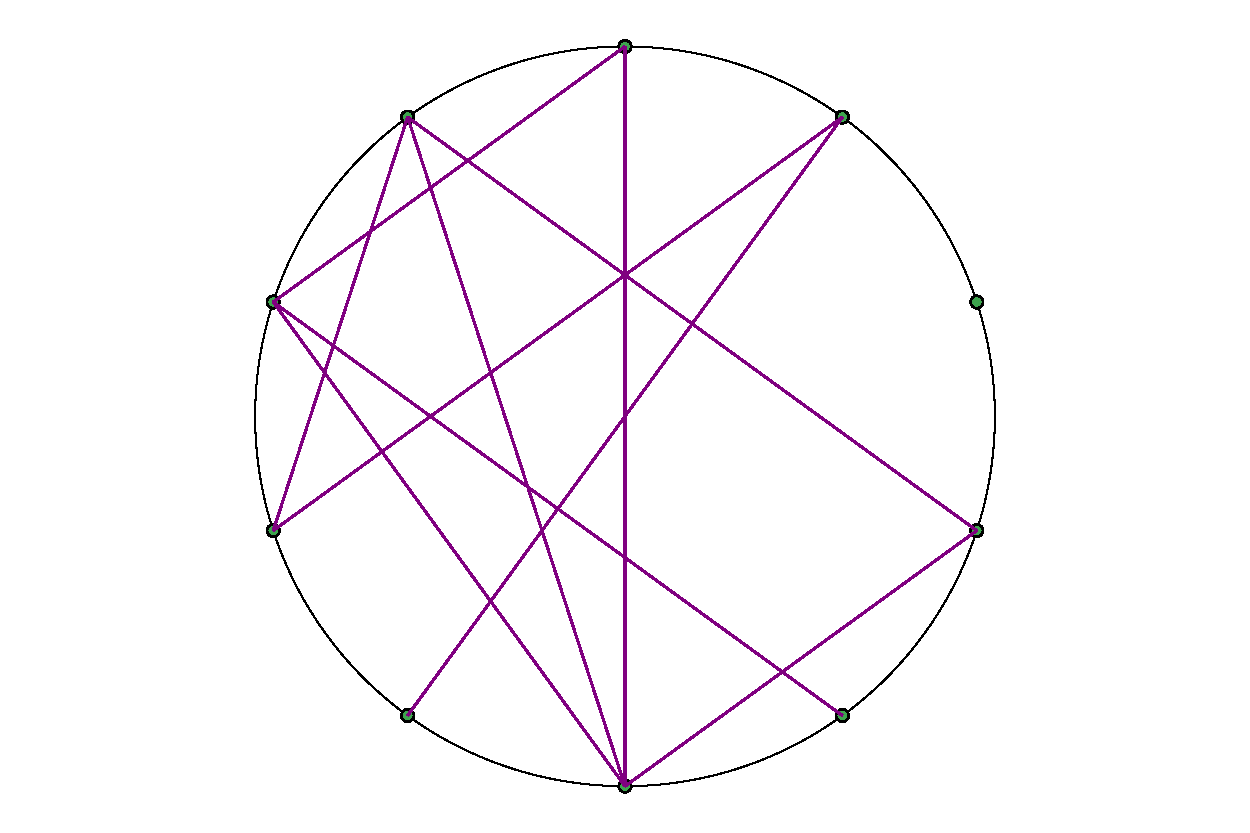
\includegraphics[width=\textwidth]{figures/partially-connected-graph.pdf}
\end{subfigure}
	\begin{subfigure}{0.5\textwidth}
	\centering
	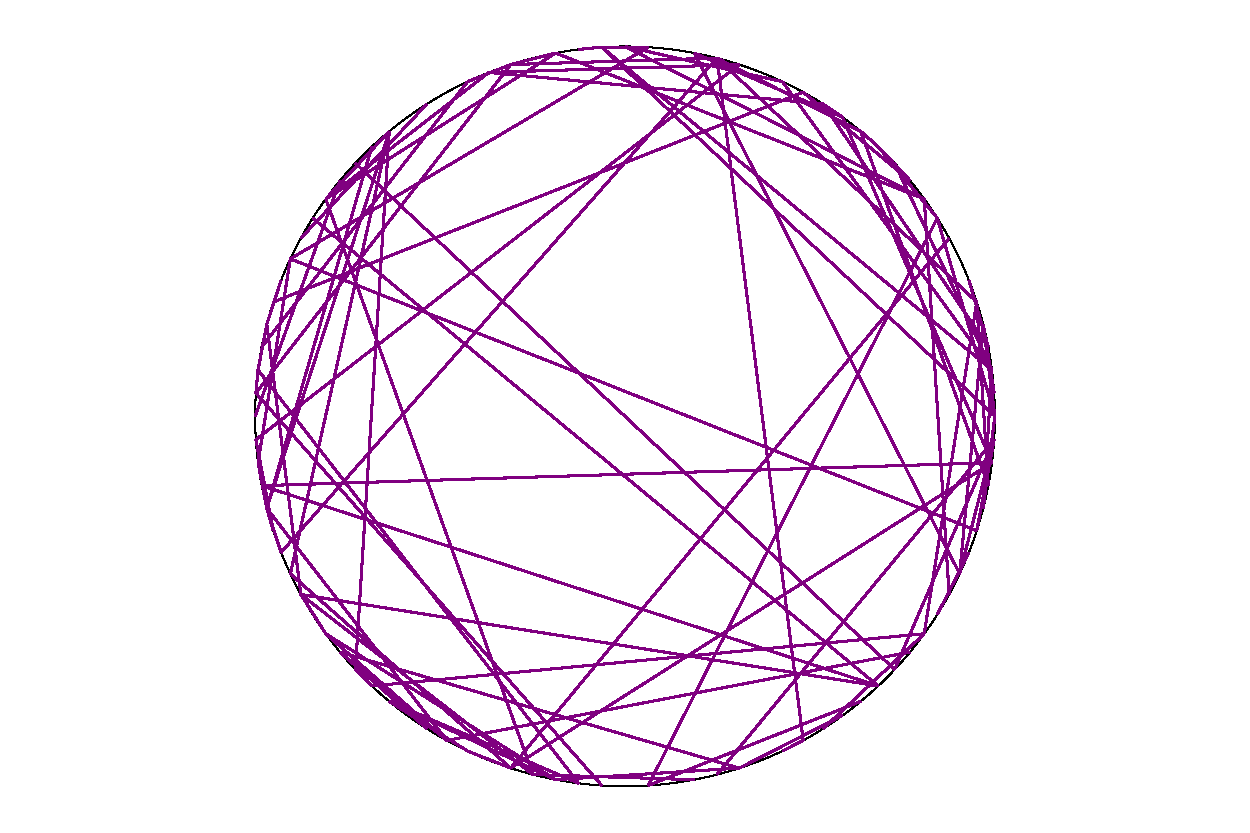
\includegraphics[width=\textwidth]{figures/partially-connected-graph-many-points-nPoints-100-nBonds-100-sigma-5.pdf}
\end{subfigure}
	\caption{Partially connected graphs of different N and $N_l$, but same $\sigma=5$. In the left panel, $N=N_l=10$, and in the right panel $N=N_l=100$.}
	\label{fig:a-partially-connected-graph}
\end{figure}

\subsection{Cluster counting}

In applying Monte Carlo algorithms to calculate thermodynamical averages, a method was introduced by \cite{PhysRevLett.58.86} in which the single spin flip seen in famous models e.g. Ising is extended to flipping whole clusters. To do so, a clustering algorithm is explained here, based on a depth first search (DFS) algorithm.

In order to apply this algorithm, the connections set must be given a new format so that the DFS algorithm can be easier applied. An array \texttt{connectionArray} of $N$ entries is created, where each of its entries is an empty array. The array \texttt{connectionArray[i]} contains the indices of the nodes to which the node \texttt{i} is connected. An example of a \texttt{connecionArray} corresponding to a fully connected graph with $N=4$ is
\begin{lstlisting}
connectionArray = [[2,3,4], [1,3,4], [1,2,4], [1,2,3].
\end{lstlisting}

The DFS algorithm is in the worst case $\mathcal{O}(V + E)$, with V the number of vertices of the graph and E the number of edges (of each cluster).  Two sets are defined
\begin{enumerate}
	\item \texttt{clusters}: The identified clusters
	\item \texttt{visited}: The visitied nodes
\end{enumerate}

Starting (arbitrarily) at the first node \texttt{n=1}. Initialize the array \texttt{stack} containing only said node, and an empty set \texttt{cluster}. Then,
\begin{enumerate}
	\item While the stack is non-empty: pop the stack to the variable \texttt{curr = pop(stack)},
	\item  If \texttt{curr} is not in \texttt{visited}, add it to \texttt{cluster}, and to the \texttt{visited} set.
	\item Retrieve the ,,neighbors'' of \texttt{curr} from \texttt{connectionArray[curr]}, and add them to the stack.
	\item Repeat step 1.
\end{enumerate}
Reaching an empty stack means there are not anymore non-visited nodes in the current cluster, and therefore \texttt{cluster} is returned and added to the set \texttt{clusters}.

The procedure is repeated for every node, if it is not in \texttt{visited}.

The corresponding \texttt{Julia} code can be found in \ref{sub:code for the clustering algorithms}.

